% !TeX root = main.tex


\chapter{State of the art and a theoretical Background}
\label{chap:2}









Chapter \ref{chap:2} introduces the theoretic baselines for data acquisition, data metrics as well as standardized data formats in which to save metadata.



Topics to consider when starting the Sensor Health Monitoring process are mainly that of providing a structured overview of the Sensor Metadata which in itself consists of many layers as a dynamically generated set of metadata is desired. This should be able to accomodate changing Data Acquisitioning (DAQ) System configuration changes.
Consideration is given to the SOIL data model and its' ability to accomodate the many demands that are expected of
sensor data management. \cite{behrens_domain-specific_2021}
The second major part to consider is that of physical crossrelations and \"deep checks\" which are a experimental mode of checking for inconsistencies among the data.
Major research and implementation work shall go into developing a dynamic model that is generated from the data and then checks back upon the data for possible discrepancies. This approach is chosen as it is estimated to be the most structured approach for a first prototype.


This topic shall give an overview over the state of the art technology as well as systems and describe the systems employed by this work. Structuring the data



\begin{figure}[h]
    \centering
    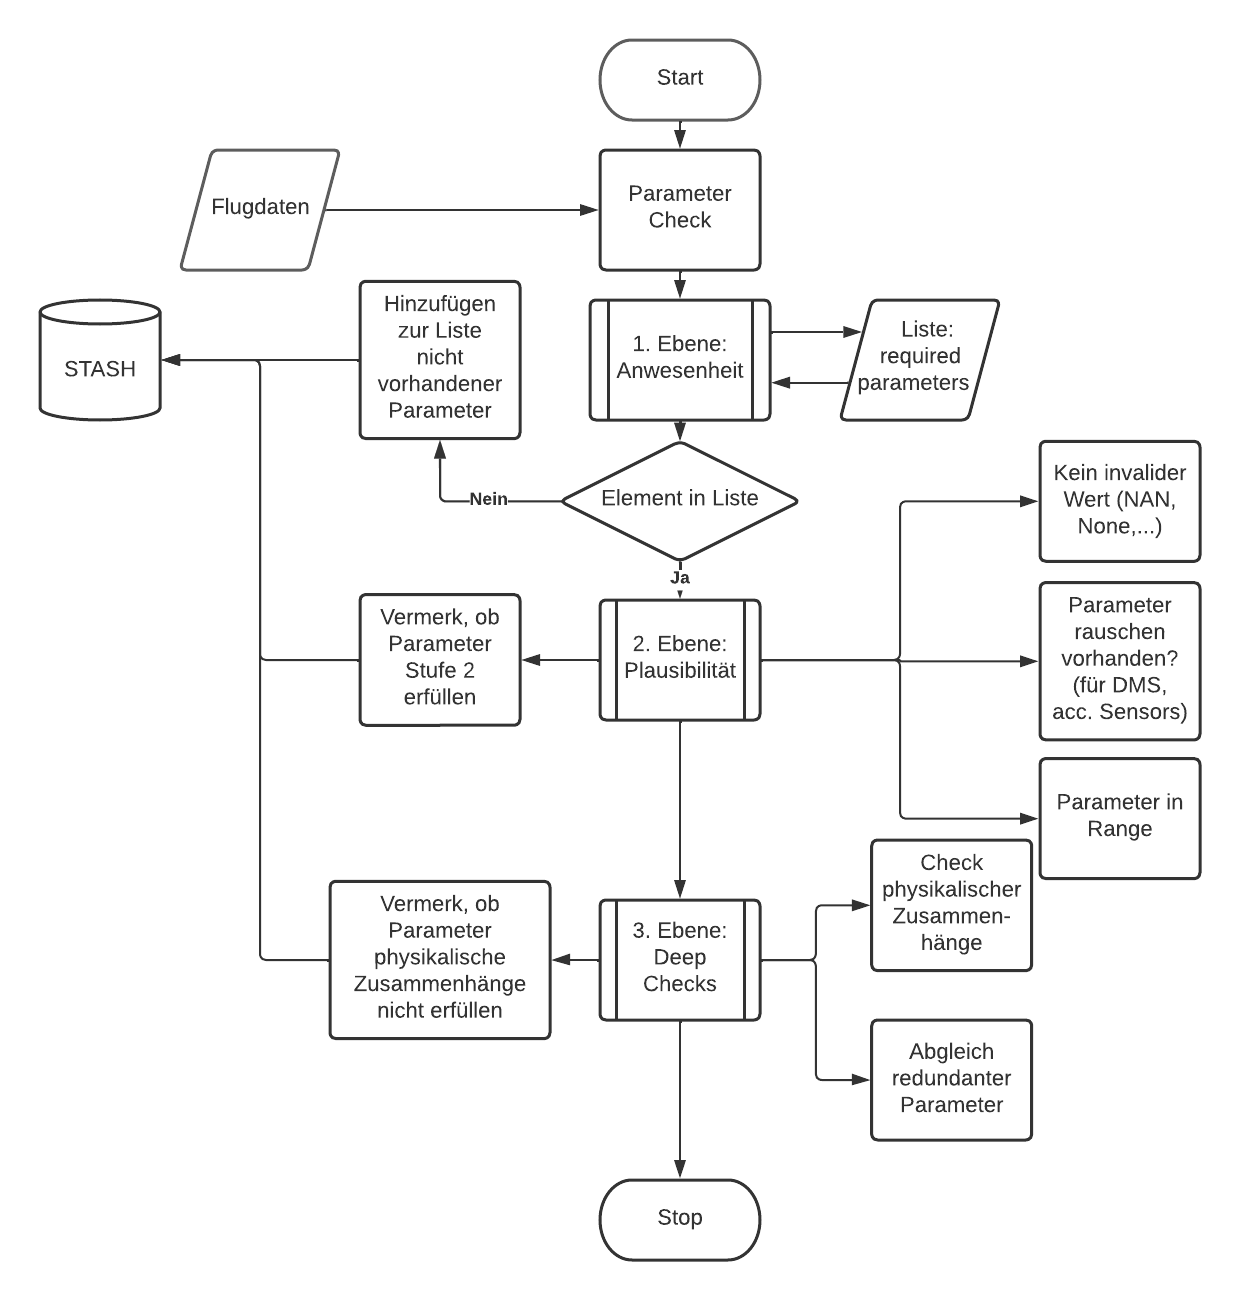
\includegraphics[width=1\textwidth]{SensorHealthMonitoring}
    \caption{}
    \label{fig:shm}
\end{figure}


\section{Data Format, FAIR}

Originating from a dutch alliance of biotechnology institutes in 2015, the FAIR Guiding principles emerged in 2016 as a general best practice guide for research data, referencing best practices

FAIR principles have been published in 2016 by the  source here. They set the foundation for a standardized and open data culture. Within these principles values like open access for data, findable and well tagged datasets, interoperable data by using standardized formats and or semantics (define semantics as well) which guarantee a reusability of data to generate a sustainable process for data usage. Effectively meaning that similar experiments do not have to be performed multiple times when well tagged and formatted data is freely available.


json file format (FAIR-principles, INST-DLR, SOIL)

Explain which means are taken to guarantee an architecture throughout the work that ensures an implementation of the FAIR principles and the V-model.
Architecture of the JSON-Tree structure and which data is inserted where.


-modern data management principles (storage not as important as readability)

Comparison with existing data structures. Implementation into existing architecture

--> Chosen Data Model, Semantics


\section{Definitions}
\begin{figure}[ht]
	\centering
	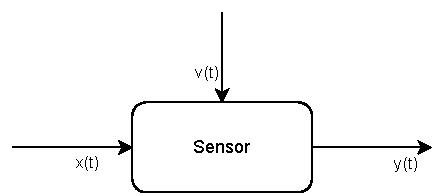
\includegraphics[width=1\textwidth]{basic_error_abb}
	\caption{Sensor Signal with control systems}
	\label{fig:basic_error_abb}
\end{figure}
\begin{figure}[ht]
	\centering
	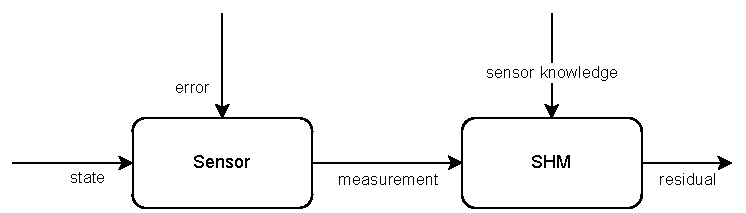
\includegraphics[width=1\textwidth]{basic_error_filter}
	\caption{Sensor Signal Filter}
	\label{fig:basic_error_filter}
\end{figure}


Unambiguous terms are needed to provide clear information within the sensor health monitoring data structure. This is needed in regards to basic terms like semantics as well as data metrics. In the following, industry standards and definitions are collected to accompany this work.

\subsection{Semantics}
Semantics are defined in various way by various people. One definition that has found some acceptance is the definition by Metzlers Lexikon which relies on theories by Blackburn and Kutschera. \cite{shoemaker_spreading_1987,kutschera_sprachphilosophie_1975}


First off, semiotics from the greek σημεῖον, semeion for sign, describes the theory of signs and their usage. Semiotics is divided into the areas semantics, syntactics and pragmatics. Within the definition at hand syntactics is given as the internal structure of signs within sign systems, pragmatics are defined as the theory of sign usage effectively thinking about how interaction with signs works.
Finally, semantics define the relationship between signs and described objects. They work by allocating a structure/model to a predefined expressions

\begin{figure}
    \centering
    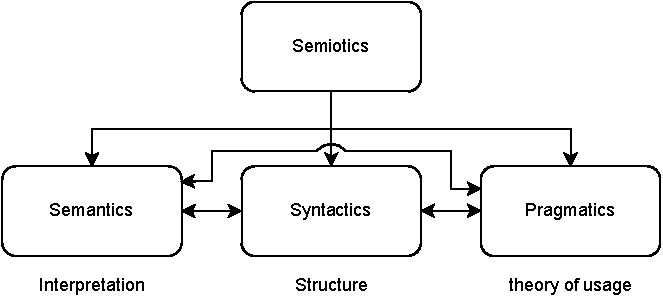
\includegraphics[width=.7\textwidth]{03_figures/semiotics.pdf}
    \caption{Semiotics, according to \textcite{kutschera_sprachphilosophie_1975} and \textcite{shoemaker_spreading_1987}}
\end{figure}

\subsection{Metadata descriptors}

No clear, fully unambiguous definition exists for most of following terms. However some assumptions have been made by e.g. isermann et al[ise97] within trends and apps.. in discussion with vdi/vde committees and the reliability, availability and maintainability (RAM) dictionary. Definitions are classified as:

deviation: difference to a reference value


\begin{itemize}
    \bfseries
    \item states and signals (chapter \ref{chap:metadata_states})
    \item functions (chapter \ref{chap:metadata_functions})
    \item models (chapter \ref{chap:metadata_models})
    \item system properties (chapter \ref{chap:metadata_system_properties})
\end{itemize}

\subsection{States and Signals}
Properties of signals

\label{chap:metadata_states}
\begin{table}[!h]
    \centering
    \begin{tabular}{@{}ll@{}}
        \toprule
        descriptor   & description                                                                           \\ \midrule
        fault        & unpermitted deviation of one subset of the system                                     \\
        failure      & permanent interruption                                                                \\
        malfunction  & intermittent regularity                                                               \\
        disturbance  & unknown, uncontrolled input                                                           \\
        perturbation & input, leading to temporary departure from steady state                               \\
        error        & deviation between measurement and true, specified, theoretically correct value        \\     & $y_e = \bar{y} -y$ \\
        residual     & fault indicator based on deviations between measurements and model-based calculations \\     & $\hat{y} = \bar{y} -y_m$ \\ \bottomrule
    \end{tabular}
    \caption{states and signals}
\end{table}

\subsection{functions}
\label{chap:metadata_functions}
\begin{table}[!h]
    \centering
    \begin{tabular}{@{}ll@{}}
        \toprule
        descriptor           & description                                                                                                     \\ \midrule
        fault detection      & determination fault presence                                                                                    \\
        fault isolation      & Determination fault properties: kind, location, time of detection                                               \\
        fault identification & determination of size and time-variant behaviour of fault                                                       \\
        fault diagnosis      & includes fault detection, isolation, identification                                                             \\
        monitoring           & real-time determination of possible physical conditions and recognition and indication of behavioural anomalies \\
        Supervision          & monitoring and taking actions to maintain operation during faults                                               \\
        protection           & means by which potentially dangerous behaviours are suppressed if possible or how consequences are avoided      \\ \bottomrule
    \end{tabular}
    \caption{functions}
\end{table}

\subsection{models}
\label{chap:metadata_models}

\begin{table}[!h]
    \centering
    \begin{tabular}{@{}ll@{}}
        \toprule
        descriptor            & description                                                                     \\ \midrule
        quantitative          & describe system in quantitative mathematical terms                              \\
        qualitative           & describe system in causalities and if-then rules                                \\
        diagnostic            & link specific inputs (symptoms) to outputs (faults)                             \\
        analytical redundancy & determine a quantity in an additional way by using a mathematical process model \\ \bottomrule
    \end{tabular}
    \caption{models}
\end{table}

\subsection{system properties}
\label{chap:metadata_system_properties}


\begin{table}[!h]
    \centering
    \begin{tabular}{@{}ll@{}}
        \toprule
        descriptor     & description          \\ \midrule
        MTTF=1/\lambda & Mean time to failure \\
        \lambda        & rate of failure      \\
        MTTR = 1/\mu   & mean time to repair  \\
        \mu            & rate of repair       \\ \bottomrule
    \end{tabular}
    \caption{system properties}
\end{table}



\begin{table}[!h]
    \centering
    \begin{tabular}{@{}ll@{}}
        \toprule
        descriptor   & description                                                                               \\ \midrule
        reliability  & ability to perform a function, measure $MTTF$, with $\lambda$ as rate of failure per hour \\
        safety       & ability of a system not to cause danger to persons, equipment and environment             \\
        availability & $A=\frac{MTTF}{MTTF + MTTR}$                                                              \\ \bottomrule
    \end{tabular}
    \caption{system properties}
\end{table}


data quality:
reliability (isermann)
availability (isermann)
accuracy

\subsection{Integrity, Reliability and Validity based on GNSS or NORMS von Lars}
Data according to ISO 8000 cite [ISO22]
iso5725:
-accuracy(validity)+precision(reliability)
Also see precision and accuracy definition \cite[S.33ff.]{smith_scientist_nodate}



Other measures for various positioning systems are found in \textcite{faa_federal_radionavigation_plan_2008}. Also, similar definitions are found as defined in \textcite{isermann_fault-diagnosis_2011}
$Reliability = 1-Probability_{Failure}$
\cite[B.1.5]{faa_federal_radionavigation_plan_2008}

B.1.10: Integrity: Display when system should not be used due to potential errors.

Validation: Black Box Testing. Results match expectations
Verification: White Box Testing. Establish algorithm's truth


\section{Signal Discretization}

State values of the real system are never measured without some error. Upon measurement, sensor values are discretized by converting it to a digital signal. This happens in two steps that are presented in an exemplary setup in figure \ref{fig:signal_processing_setup}. In the first step the real state value gets converted into a sensor signal by measuring it within a pitot tube. Within this step, some white noise generally occurs. Within the second step the sensor value gets converted to a digital signal by feeding it into an Analog Digital Converter (ADC). During the ADC step a discretization error occurs. Based upon sampling rate discretization errors occur in time and value direction. After the transformation by both steps, the data series contain a white noise sensor error as well as a discretization error (see figure \ref{fig:signal_processing_plots}, Point 3). Great effort is made to avoid such errors. For sensor errors i.e. a nose boom is fitted to the aircraft to measure undisturbed stream conditions. For value and time discretization the resolution of the ADC is chosen to guarantee necessary parameter precision. An exemplary signal transforming process is shown in figure \ref{fig:signal_processing_plots}.

\begin{figure}[!h]
    \centering
    \begin{subfigure}{\textwidth}
        \centering
        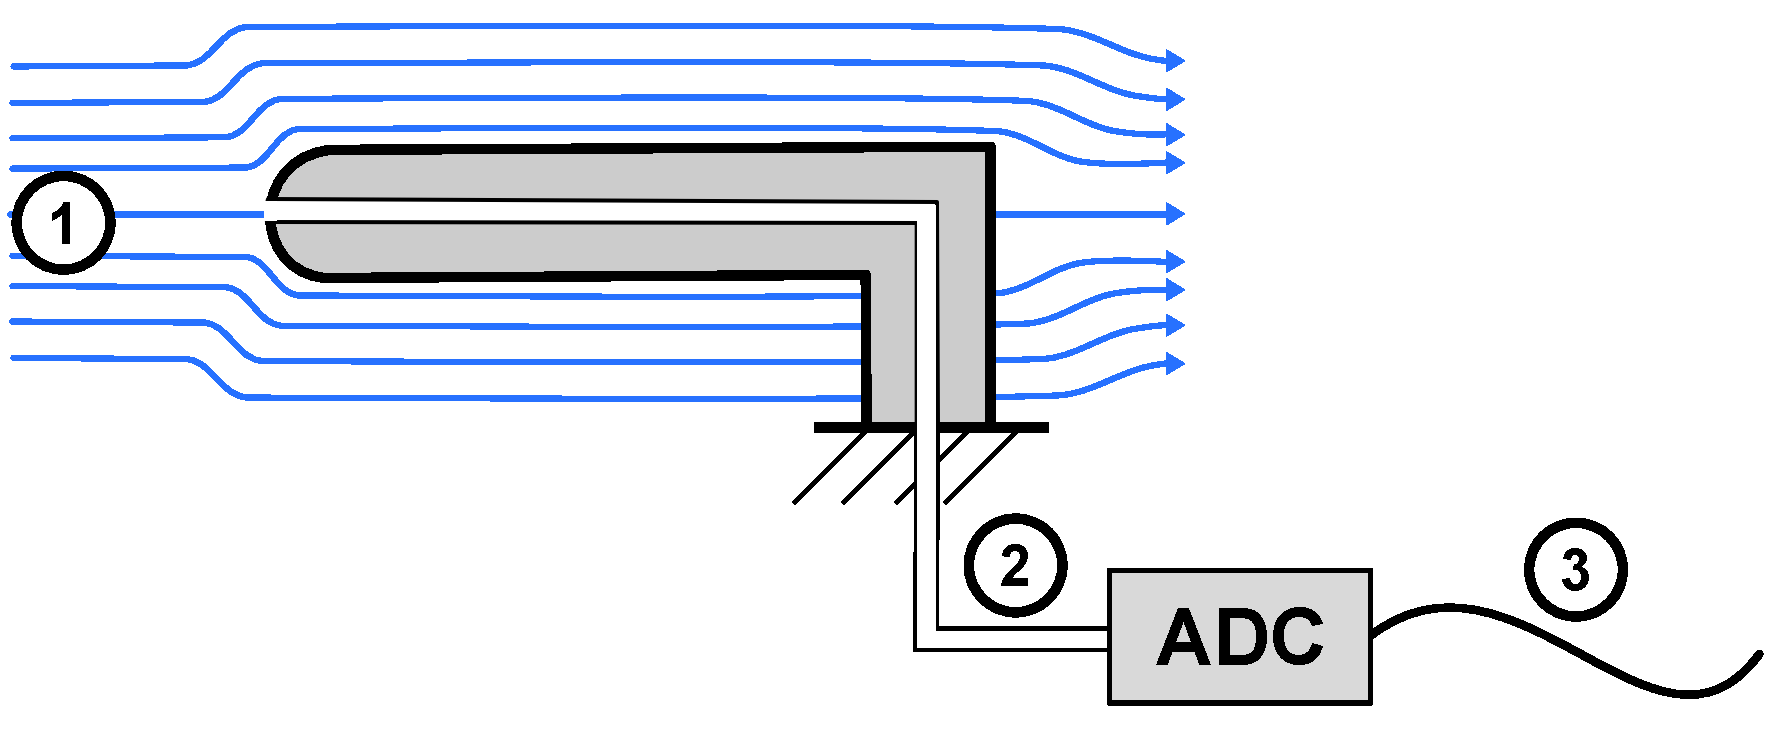
\includegraphics[width=0.8\textwidth]{03_figures/signal_recording}
        \caption{pitot tube setup for measuring dynamic pressure}
        \label{fig:signal_processing_setup}
    \end{subfigure}
    \begin{subfigure}{\textwidth}
        \centering
        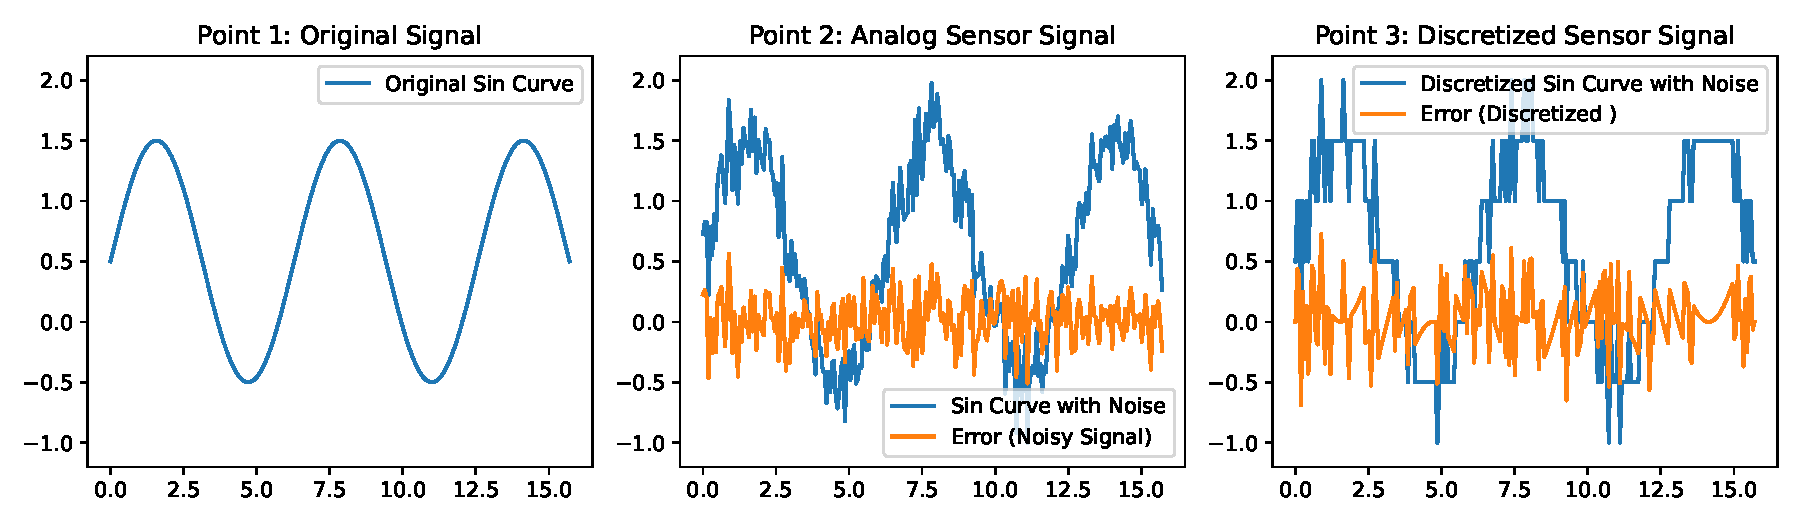
\includegraphics[width=\textwidth]{03_figures/python_functions/images/signal_processing_plots}
        \caption{Original signal into measured and discretized signal}
        \label{fig:signal_processing_plots}
    \end{subfigure}
    \caption{Simplified, exemplary signal processing flow for measurement of a dynamic pressure for real (1), analog sensor (2) and discretized sensor (3) values}
    \label{fig:signal_processing}
\end{figure}


The dynamic pressure in the air (denoted by 1) is ideally undisturbed and smooth for the actual state value. Within the sensor and stream close to the aircraft, the air is disturbed by the aircraft itself and also by the sensor, leading to the measured value at position 2. signal conversion from pressure to a voltage as well as discretization of the analog voltage to a digital signal is summarized within the ADC-Box since it is assumed that the errorwithin the pressure conversion is small compared to the errors within sensor and actual ADC. A sample signal conversion is shown within figure \ref{fig:signal_processing_plots}. Of course, errors are exaggerated for illustration since state of the art systems possess a far smaller level of sensor as well as ADC error.


All recorded sensors are present in values that are already is a process that is integral to digitally recorded sensor values.



-mention data information
-information loss through discretization

Time discretization
value quantization


\section{control systems approach}

what are state values?


Following the recipe for a modeled aircraft based on sensor data we try to simulate the parameters x and u of the aircraft with the sensor data y. Khaled shows that this approach works for linking omega_x omega_y, delta_delta(drift angle) with omega_z. and Transmissibility function  $\mathcal{T}$


The examined approaches include:
\begin{enumerate}
    \item Transmissibility functions $\mathcal{T}$ that model the system output without having to take the unknown
    system input into consideration
    \item Bond Graphs to model a physical rigid aircraft system
    \item Physical relations
    \item redundancies between sensors
\end{enumerate}

model based fault detection(isermann)
-parameter estimation (process modeling with linear or nonlinear functions, unknown process parameters are modeled by residual minimization)
-parity equations ()
-state estimation (kalman), state/output observers (for known process parameters, )
-principle component analysis


\section{Sensor Errors+SignalProperties: A quick recap(See Engineers guide to Signal Processing)}

\begin{figure}[h]
    \centering
    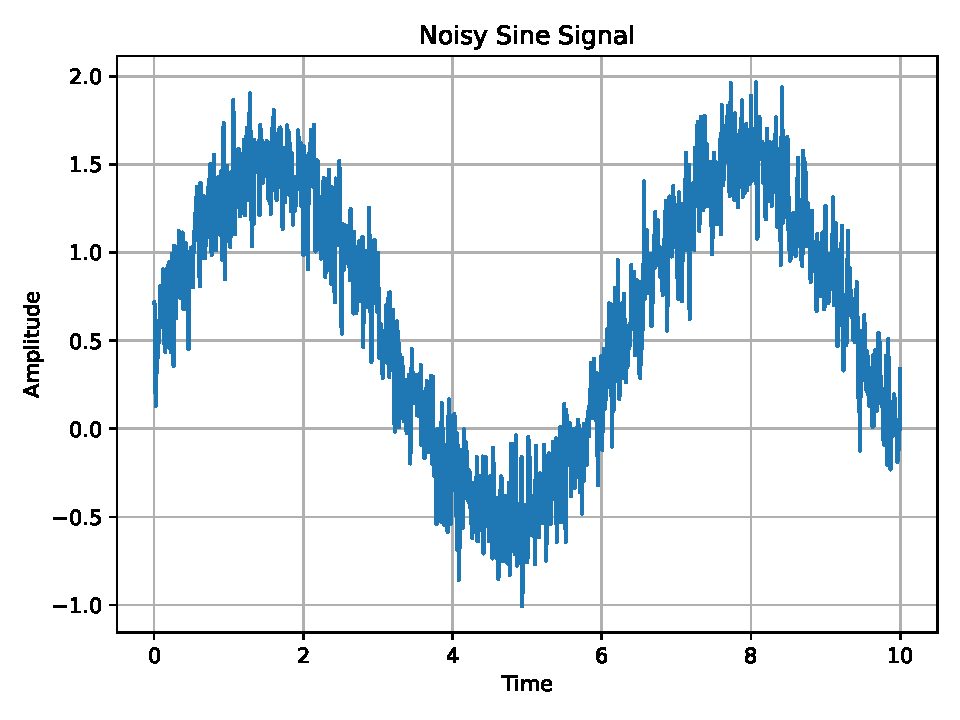
\includegraphics[width=.7\textwidth]{python_functions/images/statistic_functions_clean}
    \caption{Noisy Sine Signal}
    \label{fig:statistics_clean}
\end{figure}
\begin{figure}[h]
    \centering
    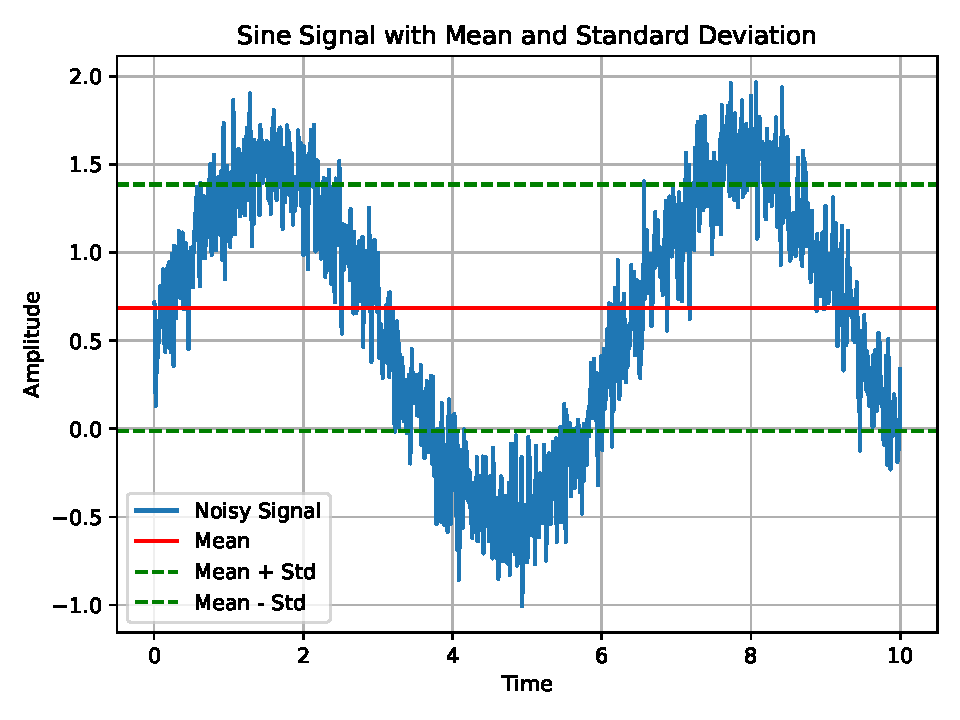
\includegraphics[width=.7\textwidth]{python_functions/images/statistic_functions_basic}
    \caption{Sine Signal with mean and standard deviation}
    \label{fig:statistics_basic}
\end{figure}
\begin{figure}[h]
    \centering
    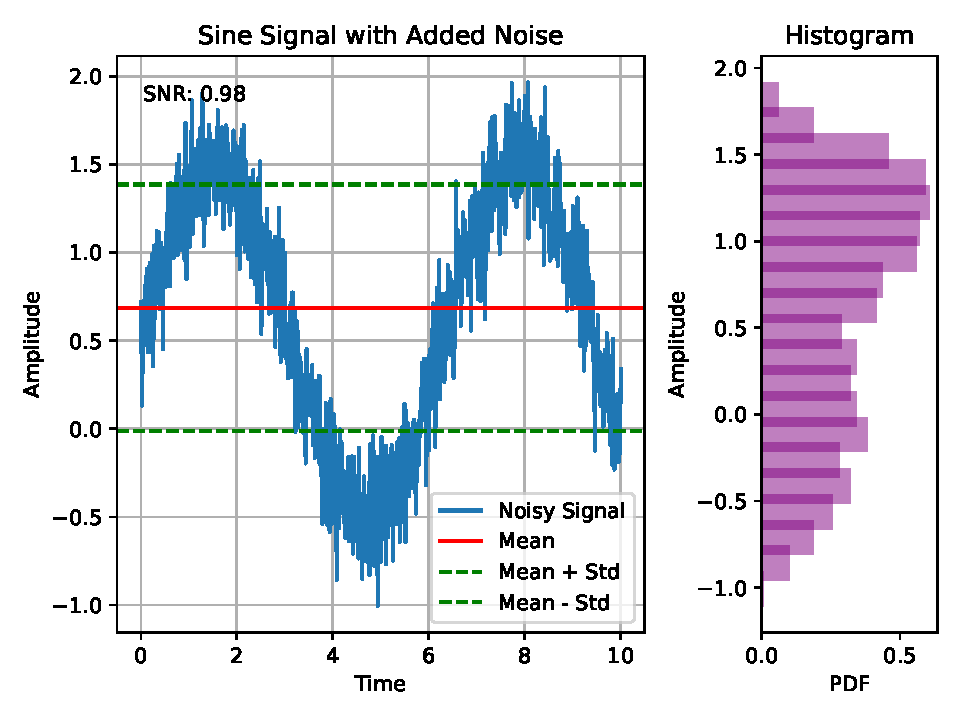
\includegraphics[width=.7\textwidth]{python_functions/images/statistic_functions_full}
    \caption{Sine Signal full analysis with mean, stdev, SNR and Histogram}
    \label{fig:statistics_full}
\end{figure}


Definition Fault Detection + Fault Diagnosis (Fault-Diagnosis Applications)


Signal properties are examined for a given signal in figure \ref{fig:statistics_clean}





Sensors generally produce errors within expected forms of output.
-Noise
-Measure using Covariance --> autocovariance
-Offset
-No response

Statistical representation of:
Mean

\cite[S.13-17]{smith_scientist_nodate}

Time continuous mean
\begin{equation}
    \label{eq:mean_cont}
    \mu=\frac{1}{T} \cdot \int_T x(t) d t
\end{equation}
Time discrete mean:
\begin{equation}
    \label{eq:mean_disc}
    \mu=\frac{1}{N} \cdot \sum_{i=1}^{N} x_i
\end{equation}




The variance $\sigma^2$ is a metric for the signal's behaviour. It expresses the mean squared deviation from the mean.

Time
\begin{equation}
    \label{eq:var_cont}
    \sigma^2=\frac{1}{T} \cdot \int_T[x(t)-\mu]^2 d t\\
\end{equation}

\begin{equation}
    \label{eq:var_disc}
    \sigma^2=\frac{1}{N} \cdot \sum_{i=0}^{N}\left[x_i-\mu\right]^2
\end{equation}

The standard deviation is derived from the variance. Its value gets square-rooted to better represent the power (magnitude of the amplitude).

Standard Deviation
\begin{equation}
    \label{eq:stdev_disc}
    \sigma = \sqrt{\sigma^2}
\end{equation}

Mean and the standard deviation don't represent the desired metrics in some use cases. Rather more important is a comparison between the two. Hence, the Signal-to-Noise ratio (SNR) is used to compare and condense the mean and standard deviation by dividing the mean by the standard deviation.

\begin{equation}
    \label{eq:snr}
    SNR=\frac{\mu}{\sigma}
\end{equation}
Another parameter is the coefficient of variation (CV) which is the standard deviation divided by the mean and multiplied by 100\%.

\begin{equation}
    \label{eq:coeff_var}
    CV = \frac{\sigma}{\mu}100\%
\end{equation}

An arising problem based on the SNR and CV are however that they scale based on the mean value. Should the mean value lie at about 0 for e.g. a sensor of an aircraft control surface, the signal to noise ratio will be relatively high compared to an acceleration sensor in z axis with a constant offset of 1g

Practical example for mean and standard deviation in a given signal are overlayed in figure \ref{fig:statistics_basic}


To evaluate a signal according to the quantities the next logical step for statistic Histogram

probability mass function

\begin{equation}
    f(x)=\frac{1}{\sqrt{2 \pi \sigma^2}} e^{-\frac{(x-\mu)^2}{2 \sigma^2}}
\end{equation}


Covariance
Zeitkontinuierliche Autokovarianzfunktion
$$
\gamma(\tau)=\frac{1}{T} \cdot \int_T[x(t)-\mu] \cdot[x(t-\tau)-\mu] d t
$$
Zeitdiskrete Autokovarianzfunktion
$$
\gamma(k)=\frac{1}{N} \cdot \sum_N\left[x_i-\mu\right] \cdot\left[x_{i-k}-\mu\right]
$$

-->Autocovariance
autocov(x,x) = cov(x,x)


Correlation (Pearson coefficient)

$$\rho_{x,y} = corr(x,y)=\frac{cov(x,y)}{\sigma_x \sigma_y}$$

Total correlation 1 or negative correlation -1.

Total independence for $\rho_{x,y}=0$ not given since Pearson coefficient only detects linear correlations

Other correlation methods as rank-correlation (Spearman, Kendall) that detect change correlations are possible but are more complex in the implementation.


stft.

Test noise analysis over short time window of 256 samples.

Define here


Also, next to the simple and known models to display an error is the Luenberger Beobachter.
enter placeholder for image: Measurement equals signal + error
and image: luenberger beobachter. Kalman Implementierung (Lie13)
Parameter Correlation Studies (Li15)


\section{Faults}
Offset, bias, hysteresis from literature

Fault definition from [fmea? Isermann(20)]
primary and secondary data (\cite{giez_determination_2022})


\section{Intro existing architectures}
Sensor data is presently already generated and uploaded to the skystash architecture described in chapter \ref{chap:skystash} while it is uploaded


\section{DAQs, ISTAR}
DLR data generation (DAQs) (How Data is checked)

Matthews flowchart(dataflow from sensor voltage through computer-computer-user)
Exemplary for a single sensor.

The ISTARs DAQ records the aircrafts own flight data bus (ASCB, avionics standard communications bus), the experimental Noseboom, an additional GPS unit and various additional strain gauges and acceleration sensors that are distributed across the aircraft. configuration currently is described differently within each sub-group.


\section{skystash}
\label{chap:skystash}

dlrk paper hier zitieren.

\begin{figure}[h]
    \centering
    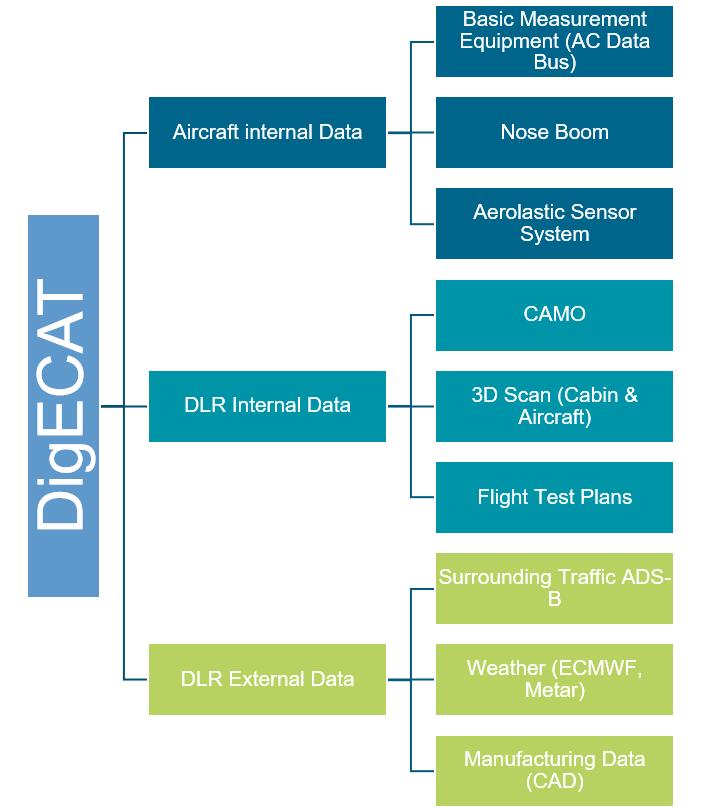
\includegraphics{03_figures/DIGECAT}
    \caption{Generation of flight test data }
\end{figure}

\begin{figure}[h]
    \centering

\end{figure}

the skystash is a platform to distribute, analyze and visualize large flight data sets. It is currently in development within the DLR's digital twin project and aims to be a service platform for uploading and sharing the DLR's flight test data. Various requirements are posed from different sources such as flight guidance projects that are content with sampling rates as 1 Hz and aeroelastic examinations that receive sampling rates of 2000Hz. For this purpose a dynamic data export is sensible in which users can directly choose sampling rates as well as single parameters from a flight contrary to downloading and working with a whole flight data set averaging up to 2GB of data.

This work builds upon the python api and tries to implement and test an algorithm that checks the data for the istar aircraft


\section{downloadfunctionalities}
file sizes too large --> Reduction for on demand parameters and resampling utility
Handling of large data sets


\section{Deep dive into altitudes}

The aircraft altitude generally is defined as the displacement of the aircraft from sea level.
On a geodetic scale, the earth can be described as an ellipsoid due to its rotation. However, varying density levels of the earth's crust cause the elevation and sea level to deviate from the ellipsoid shape. This results in a lopsided model that is modeled in the WGS84 (ref and image here) system. This is also the altitude that the gps measures. And will be the reference altitude for the following calculations.

The main existing altitudes are the:
\begin{enumerate}
    \item Geodetic Altitude (GNSS)
    \item Barometric Altitude (used in conjunction with reference pressure)
    \item Inertial Altitude
    \item Radar Altitude (can be used in conjunction with a terrain model to derive geodetic altitude)
\end{enumerate}
Possible errors for each are:
geodetic: inconvenient satellite placements, deflection of signals in the atmosphere and signal problems
Barometric Altitude: Possible errors due to drift and meteorological atmospherical pressure shifts, Reference Altitude.

Going into WGS84 and the GNSS Altitude however exceeds the scope of this work. In the following, the satellite altitude above Mean Sea Level (MSL) is considered as the reference altitude.


\section{gnss algorithms}

Fault detection algorithms within GNSS are described as Receiver Autonomous Integrity Monitoring (RAIM) are tried and tested within GNSS implementations since high accuracy positioning is valuable for various applications, reaching precisions of up to a few centimeters. Explaining the full function of position calculation exceeds this works' scope. To summarize however, GNSS inputs form an overdefined system of equations which needs to be compensated within some algorithm to form one position based on multiple inputs.


ica18 annex10
ABAS, RAIM, AAIM
